\documentclass[a4paper,10pt]{article}
\usepackage[utf8]{inputenc}


\usepackage{graphicx}
\usepackage{theorem}        %%Lo agregue yo <========================================
\usepackage{algorithm}      %%Lo agregue yo <========================================
\usepackage{algorithmic}        %%Lo agregue yo <========================================
\usepackage{amssymb, amsmath}



\newtheorem{mytheorem}{Theorem}
\newtheorem{example}{Example}[section]  %\newtheorem{ambiente}{título}[numeração] 
\newtheorem{definition}[mytheorem]{Definition}
\newtheorem{mylemma}[mytheorem]{Lemma}
\newenvironment{myproof}[1][Proof]{\textbf{#1.} }{\ \rule{0.5em}{0.5em}}

%%%%%%%%%%%%%%%%%%%%%%%%%%%%%%%%%%%%%%%%%%%%%%%%%%%%%%%%%%%%%%%%%%%%%%%%%%%

\usepackage{color}                          % colors
\usepackage{framed}                         % frames
\usepackage{mdframed}                       % better frames
\usepackage{fancyhdr}                       % Fancy headings

\definecolor{thmBgColor}{RGB}{250,250,250}
\definecolor{thmLnColor}{RGB}{200,200,200}

\mdfdefinestyle{MDFStyGrayScreen}{%
    linecolor=thmLnColor,
        backgroundcolor=thmBgColor,
        linewidth=1pt,
        topline=true,
    bottomline=true,
    rightline=false,
        leftline=false,
    outerlinewidth=2pt,
    roundcorner=0pt,
    innertopmargin=4pt, %\baselineskip
    innerbottommargin=4pt, %\baselineskip,
    innerrightmargin=3pt,
    innerleftmargin=3pt,
        skipabove=\topskip,
        skipbelow=\topskip,
        nobreak=true
        }
%%%%%%%%%%%%%%%%%%%%%%%%%%%%%%%%%%%%%%%%%%%%%%%%%%%%%%%%%%%%%%%%%%%%%%%%%%%

%opening
\title{Demonstrations Database}
\author{Fernando Pujaico Rivera}

\begin{document}

\maketitle

\begin{abstract}
This article have a set of demonstrations necessary for other articles
\end{abstract}

\section{System Model}
\label{Sec:system}

System model of system studied in this article in Fig. \ref{fig:Model}, where
$Pr(U_0=1)=0.5$ then consequently $Pr(U_m=1)=0.5$ $\forall m \in \{1, ..., M\}$.
\begin{figure}[h!bt]
\centering 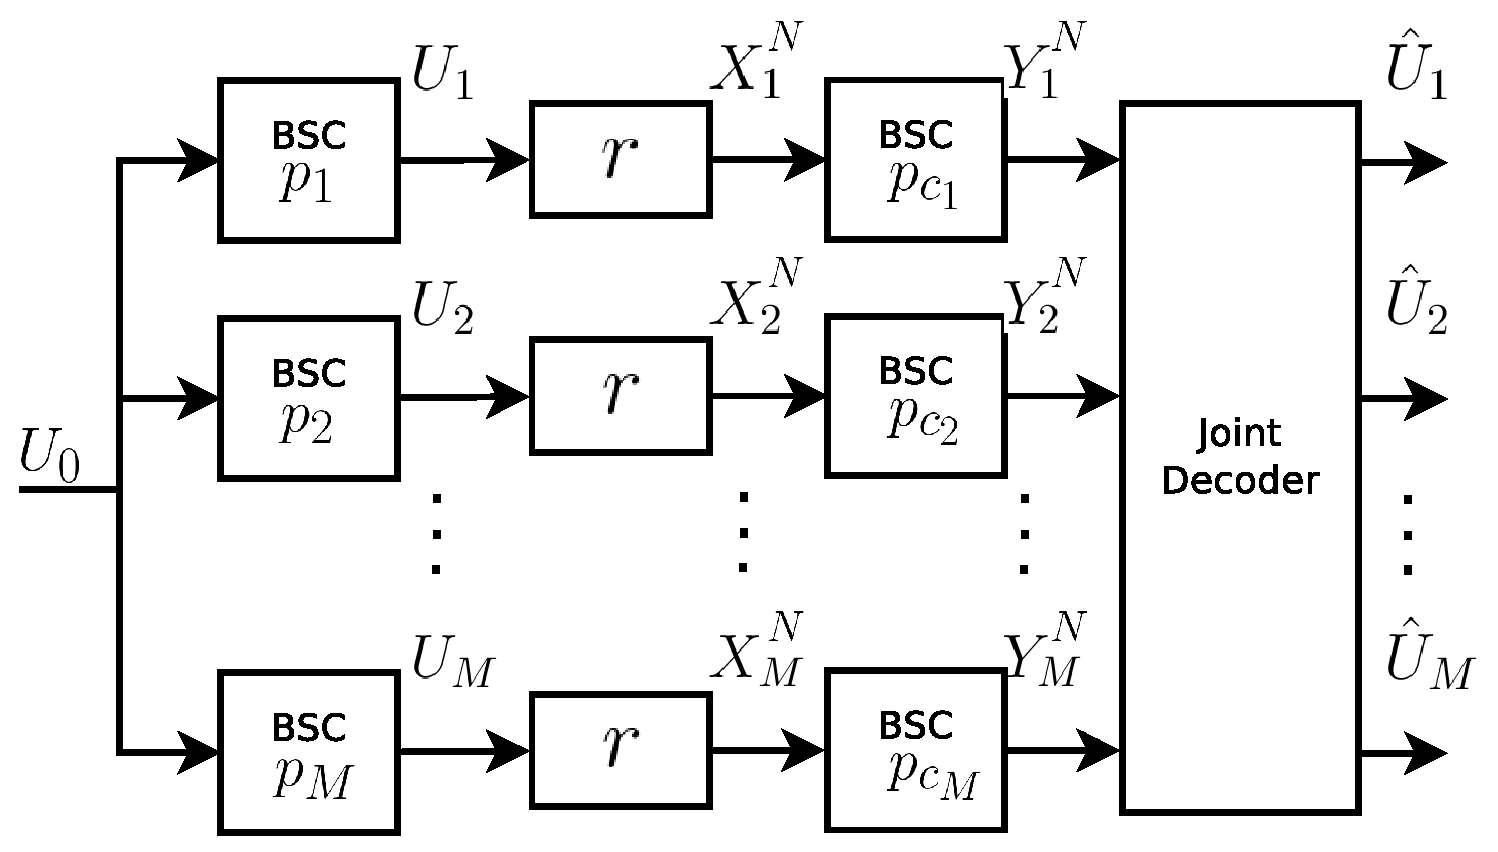
\includegraphics[width=12cm]{{./fig1.eps}}
\caption{System model.}
\label{fig:Model}
\end{figure}

\section{Demonstrations}
\label{Sec:Demons}



%%%%%%%%%%%%%%%%%%%%%%%%%%%%%%%%%%%%%%%%%%%%%%%%%%%%%%%%%%%%%%%%%%%%%%%%%%%%%%
\begin{definition}
 \label{def:omega}
Let $\Omega_m$, $\forall m \in \{1,$ $2,$ $...,$ $M\}$, be a set of correlated 
sources as
\begin{equation}
\label{eq:omega}
 \Omega_m \equiv U_1 U_2 ... U_m,
\end{equation}
with the especial case with $\Omega_0$ equal to null,
where each source $U_i$, $\forall$ $i \in$ $\{1,$ $2,$ $...,$ $m\}$, is created 
passing the source $U_0$, $Pr(U_0=1)=0.5$, across a BSC channel  with error 
probability $Pr(U_i \ne U_0 | U_0)=p_i$.

In this line, also is defined a set of correlated sources $\Omega^{M}_m$, 
$\forall m \in \{1,$ $2,$ $...,$ $M\}$, as anything set of $m$  sources in $\Omega_M$, 
with the especial case with $\Omega^M_0$ equal to null.
\end{definition}

%%%%%%%%%%%%%%%%%%%%%%%%%%%%%%%%%%%%%%%%%%%%%%%%%%%%%%%%%%%%%%%%%%%%%%%%%%%%%%
\begin{definition}
 \label{def:hb}
The binary entropy is defined as $h_b(\rho)$, such that
\begin{equation}
\label{eq:hb1}
h_b(\rho)=- \rho ~ log_2(\rho) - (1-\rho) ~ log_2(1-\rho).
\end{equation}
If the probability $p_m$ is used, then is defined
\begin{equation}
\label{eq:hi}
h_m \equiv h_b(p_m)
\end{equation}
\end{definition}

%%%%%%%%%%%%%%%%%%%%%%%%%%%%%%%%%%%%%%%%%%%%%%%%%%%%%%%%%%%%%%%%%%%%%%%%%%%%%%
%%%%%%%%%%%%%%%%%%%%%%%%%%%%%%%%%%%%%%%%%%%%%%%%%%%%%%%%%%%%%%%%%%%%%%%%%%%%%%
\begin{mdframed}[style=MDFStyGrayScreen]
\begin{mylemma}
\label{lemma:def} 
If we defined 
\begin{equation} \label{eq:ab2}
 p_a || p_b \equiv p_a + p_b -2 p_a p_b, 
\end{equation} 
then the operator $||$ is an associative operator such that
\begin{equation} \label{eq:def1}
 (p_a || p_b)||p_c = p_a || (p_b||p_c)
\end{equation} 
\end{mylemma}
\end{mdframed}
\begin{myproof}
\label{proof:def}
\begin{equation} \label{eq:def2}
\begin{matrix}
(p_a || p_b)||p_c & = & p_a + p_b + p_c -2 p_a p_b -2 p_b p_c  \\
~                 & ~ & -2 p_a p_c + 4 p_a p_b p_c.
\end{matrix}
\end{equation} 
If we developing similarly $p_a || (p_b||p_c)$ we reached the same result, and 
the Lemma \ref{lemma:def} is proved.
\end{myproof}
%%%%%%%%%%%%%%%%%%%%%%%%%%%%%%%%%%%%%%%%%%%%%%%%%%%%%%%%%%%%%%%%%%%%%%%%%%%%%%
%%%%%%%%%%%%%%%%%%%%%%%%%%%%%%%%%%%%%%%%%%%%%%%%%%%%%%%%%%%%%%%%%%%%%%%%%%%%%%
\begin{mdframed}[style=MDFStyGrayScreen]
\begin{mylemma}
\label{lemma:psimple} 
Known 2 probabilities $p_1$, and $p2$
them is true that
\begin{equation} \label{eq:psimple1}
h_b(p_1) \leq h_b(p_1||p_2) 
\end{equation}
\end{mylemma}
\end{mdframed}
\begin{myproof}
\label{proof:psimple} 
We know  by Jensen's inequality \cite{cover} that for a concave function $f(.)$ 
is true that
\begin{equation} \label{eq:psimple2}
(1-\lambda) f(p_1) +\lambda f(1-p_1)  \leq f((1-\lambda) p_1 +\lambda (1-p_1))
\end{equation}
replacing the function $f(.)$ by the concave function $h_b(.)$ and $\lambda$ 
by $p_2$ we obtain
\begin{equation} \label{eq:psimple3}
h_b(p_1)  \leq h_b(p_2 + p_1 - 2 p_1 p_2)
\end{equation}
and the lemma is proved.
%and finally
%\begin{equation} \label{eq:psimple4}
%h_b(p_1)  \leq h_b(p_1|| p_2).
%\end{equation}
\end{myproof}
%%%%%%%%%%%%%%%%%%%%%%%%%%%%%%%%%%%%%%%%%%%%%%%%%%%%%%%%%%%%%%%%%%%%%%%%%%%%%%
%%%%%%%%%%%%%%%%%%%%%%%%%%%%%%%%%%%%%%%%%%%%%%%%%%%%%%%%%%%%%%%%%%%%%%%%%%%%%%
\begin{mdframed}[style=MDFStyGrayScreen]
\begin{mylemma}
\label{lemma:ppapb} 
Known 3 probabilities $p_a$, $p_b$ and $p$, where
\begin{equation} \label{eq:ppapb0}
h_b(p_a) \leq h_b(p_b) 
\end{equation}
them is true that
\begin{equation} \label{eq:ppapb1}
h_b(p||p_a) \leq h_b(p||p_b) 
\end{equation}
\end{mylemma}
\end{mdframed}

\begin{myproof}
\label{proof:ppapb} 
Using the Lemma \ref{lemma:def} and \ref{lemma:psimple}, and replacing 
$p_1$ by $p || p_a$, the equation (\ref{eq:psimple1}) can be rewrite as 
\begin{equation} \label{eq:ps1}
h_b(p || p_a) \leq h_b(p|| (p_a||p_2)).
\end{equation}
If we call to $p_a||p_2$ as $p_b$, and it is replace in (\ref{eq:ps1}) we obtain
the same equation that in (\ref{eq:ppapb1}) and the lemma is proved.
\end{myproof}
%%%%%%%%%%%%%%%%%%%%%%%%%%%%%%%%%%%%%%%%%%%%%%%%%%%%%%%%%%%%%%%%%%%%%%%%%%%%%%
%%%%%%%%%%%%%%%%%%%%%%%%%%%%%%%%%%%%%%%%%%%%%%%%%%%%%%%%%%%%%%%%%%%%%%%%%%%%%%
\begin{mdframed}[style=MDFStyGrayScreen]
\begin{mylemma}
\label{lemma:twoparbsc}
Known two correlated binary sources $U_a$ and $U_b$ that are created passing 
the binary source $U_0$, $Pr(U_0=1)=0.5$, through of two BSC channels with  
error probabilities $p_a$ and $p_b$ respectively. These can be modeled as a 
source $U_b$ that is created passing the source $U_a$ through of one BSC 
channel with  error probability 
\begin{equation} \label{eq:tpb0}
Pr(U_b \neq U_a|U_a)=P_a || P_b.
\end{equation}
\end{mylemma}
\end{mdframed}

\begin{myproof}
\label{proof:twoparbsc}
The equation (\ref{eq:tpb0}) imply to prove that 
\begin{equation} \label{eq:tpb1}
Pr(U_b=1|U_a=0)=Pr(U_b=0|U_a=1).
\end{equation}
Development both parts we obtain
\small
\begin{equation} \label{eq:tpb2}
\begin{matrix}
Pr(U_b=1|U_a=0) & = & \frac{Pr(U_b=1,U_a=0)}{Pr(U_a=0)}\\ 
 ~              & = & \frac{Pr((U_b=1,U_a=0)|U_0=0)Pr(U_0=0)}{Pr(U_a=0)}\\ 
 ~              & + & \frac{Pr((U_b=1,U_a=0)|U_0=1)Pr(U_0=1)}{Pr(U_a=0)}\\
 ~              & = & \frac{Pr(U_b=1|U_0=0)Pr(U_a=0|U_0=0)Pr(U_0=0)}{Pr(U_a=0)}\\ 
 ~              & + & \frac{Pr(U_b=1|U_0=1)Pr(U_a=0|U_0=1)Pr(U_0=1)}{Pr(U_a=0)}\\
 ~              & = & p_b(1-p_a)+(1-p_b)p_a\\ 
 ~              & = & p_a+p_b -2 p_a p_b,
\end{matrix}
\end{equation}
\normalsize
in the other hand similarly to (\ref{eq:tpb2}) we obtain that 
$Pr(U_b=1|U_a=1)=P_a || P_b$. Thus, the Lemma \ref{lemma:twoparbsc} is proved.
\end{myproof}
%%%%%%%%%%%%%%%%%%%%%%%%%%%%%%%%%%%%%%%%%%%%%%%%%%%%%%%%%%%%%%%%%%%%%%%%%%%%%%
%%%%%%%%%%%%%%%%%%%%%%%%%%%%%%%%%%%%%%%%%%%%%%%%%%%%%%%%%%%%%%%%%%%%%%%%%%%%%%
\begin{mdframed}[style=MDFStyGrayScreen]
\begin{mylemma}
\label{lemma:minimo}
We consider that have $\hat{\Omega}_{m}$ as a set of sources that pertain 
$\Omega_M$, also $U_{a}$ and $U_b$, $\forall b \geq {a}$, are sources that 
pertain to $\Omega_M$ but not to $\hat{\Omega}_{m}$, such that $ h_b(p_a) \leq h_b(p_b)$
then
\begin{equation}\label{eq:proof1}
 H(\hat{\Omega}_{m} U_{a} ) \leq H(\hat{\Omega}_{m} U_b ),
\end{equation}
\end{mylemma}
\end{mdframed}

\begin{myproof}
\label{proof:minimo}
The equation (\ref{eq:proof1}) is equivalent to
\begin{equation}\label{eq:proof2}
 H( U_{a}| \hat{\Omega}_{m}) \leq H(U_b| \hat{\Omega}_{m} ).
\end{equation} 
$\hat{\Omega}_{m}$  only have a relation with $U_a$ and $U_b$ through of $U_0$. The
known of $\hat{\Omega}_{m}$ only give a distorted known of source $U_0$, this
distorted source is called here as $\tilde{U}_0$ and can be modeled as
 if the source $\tilde{U}_0$ was created passing the source $U_0$ through of
a BSC channel with error probability $p_{\hat{\Omega}_{m}}$, that only depend of 
$\hat{\Omega}_{m}$. Thus, the equation (\ref{eq:proof2}) can be rewrite as 
\begin{equation}\label{eq:proof3}
 H( U_{a}| \tilde{U}_0) \leq H(U_b| \tilde{U}_0 ).
\end{equation} 
Using the Lemma \ref{lemma:twoparbsc} the last equation can be rewrite as
\begin{equation}\label{eq:proof4}
h_b( p_{\hat{\Omega}_{m}}||p_{a} ) \leq h_b( p_{\hat{\Omega}_{m}}||p_{b} ).
\end{equation} 
For definition of problem we know that $h_b(p_a) \leq h_b(p_b)$. Using the 
Lemma \ref{lemma:ppapb}, we can demonstrate that (\ref{eq:proof4}) is true
and consequently (\ref{eq:proof1}) to. 
\end{myproof}
%%%%%%%%%%%%%%%%%%%%%%%%%%%%%%%%%%%%%%%%%%%%%%%%%%%%%%%%%%%%%%%%%%%%%%%%%%%%%%
%%%%%%%%%%%%%%%%%%%%%%%%%%%%%%%%%%%%%%%%%%%%%%%%%%%%%%%%%%%%%%%%%%%%%%%%%%%%%%
\begin{mdframed}[style=MDFStyGrayScreen]
\begin{mylemma}
 \label{lemm:PrA}
Known a set of $m$ correlated  sources  $\Omega_m$. Then, is true that
\begin{equation}\label{eq:PA}
Pr(\Omega_m=\mathbf{a})=\frac{ \Psi(\mathbf{a}) + \Psi(\mathbf{\bar{a}}) }{2},
\end{equation}
\begin{equation}\label{eq:PAequiv}
\Psi(\mathbf{a}) \equiv \prod \limits_{i=1}^{m}{Pr(U_i=a_i|U_0=0)}.
\end{equation}
being $\mathbf{a}=\{a_1, a_2, ..., a_m\}$ and $\mathbf{\bar{a}}$ two 
binary vectors, both with $m$ elements, where $\mathbf{\bar{a}}\oplus \mathbf{a}=\mathbf{0}$. 
\end{mylemma}
\end{mdframed}

\begin{myproof}
 \label{proof:PrA} 
\begin{equation}\label{eq:PA1}
\begin{matrix}
Pr(\Omega_m=\mathbf{a})&=&Pr(\Omega_m=\mathbf{a}|U_0=0)Pr(U_0=0)\\
~                 &+&Pr(\Omega_m=\mathbf{a}|U_0=1)Pr(U_0=1), 
\end{matrix}
\end{equation}
\begin{equation}\label{eq:PA2}
Pr(\Omega_m=\mathbf{a})=\frac{Pr(\Omega_m=\mathbf{a}|U_0=0)+Pr(\Omega_m=\mathbf{a}|U_0=1)}{2},
\end{equation}
when $U_0$ is known the probabilities of sources in $\Omega_m$ are independents,
\begin{equation}\label{eq:PA3}
Pr(\Omega_m=\mathbf{a})=\frac{\prod \limits_{U_i\in \Omega_m}{Pr(U_i=a_i|U_0=0)}+\prod \limits_{U_i\in \Omega_m}{Pr(U_i=a_i|U_0=1)}}{2},
\end{equation}
\end{myproof}
%%%%%%%%%%%%%%%%%%%%%%%%%%%%%%%%%%%%%%%%%%%%%%%%%%%%%%%%%%%%%%%%%%%%%%%%%%%%%%
%%%%%%%%%%%%%%%%%%%%%%%%%%%%%%%%%%%%%%%%%%%%%%%%%%%%%%%%%%%%%%%%%%%%%%%%%%%%%%
\begin{mdframed}[style=MDFStyGrayScreen]
\begin{mylemma}
 \label{lemm:dhdrho}
Known the binary entropy $h(\rho)=-\rho log_2(\rho)-(1-\rho) log_2(1-\rho)$ then
\begin{equation}\label{eq:dhdrho1}
 \frac{\partial h(\rho)}{\partial \rho}= log_2 \left( \frac{1-\rho}{\rho} \right )
\end{equation}
\end{mylemma}
\end{mdframed}

\begin{myproof}
 \label{proof:dhdrho} 
\begin{equation}\label{eq:dhdrho2}
 \frac{\partial h(\rho)}{\partial \rho}= - log_2(\rho)+ log_2(1-\rho)
\end{equation}
\end{myproof}
%%%%%%%%%%%%%%%%%%%%%%%%%%%%%%%%%%%%%%%%%%%%%%%%%%%%%%%%%%%%%%%%%%%%%%%%%%%%%%
%%%%%%%%%%%%%%%%%%%%%%%%%%%%%%%%%%%%%%%%%%%%%%%%%%%%%%%%%%%%%%%%%%%%%%%%%%%%%%
\begin{mdframed}[style=MDFStyGrayScreen]
\begin{mylemma}
 \label{lemm:dH}
Known a set of $m$ correlated  sources  $\Omega_m$. Then, is true that
the value of entropy $H(\Omega_m)$ grow in relation growing of $h_b(p_i)$, 
$\forall i$ $\in \{1,$ $2,$ $...,$ $m\}$,
\begin{equation}\label{eq:dH1}
 \frac{\partial H(\Omega_m)}{\partial h_i} \geq 0
\end{equation}
\end{mylemma}
\end{mdframed}

\begin{myproof}
 \label{proof:dH} 
\begin{equation}\label{eq:dH2}
 \frac{\partial H(\Omega_m)}{\partial h_i} =\frac{\partial \sum -Pr(\Omega_m=\mathbf{a}) log_2(Pr(\Omega_m=\mathbf{a}))}{\partial h_i} 
\end{equation}
\end{myproof}
%%%%%%%%%%%%%%%%%%%%%%%%%%%%%%%%%%%%%%%%%%%%%%%%%%%%%%%%%%%%%%%%%%%%%%%%%%%%%%
%%%%%%%%%%%%%%%%%%%%%%%%%%%%%%%%%%%%%%%%%%%%%%%%%%%%%%%%%%%%%%%%%%%%%%%%%%%%%%
\begin{mdframed}[style=MDFStyGrayScreen]
\begin{mylemma}
 \label{lemm:H}
 Known a system model as Fig. \ref{fig:Model}, then
  \begin{equation}\label{eq:H}
H(\Omega_m) = \sum_{i=1}^{m}{h_b(p_i)}+1-H(U_0|\Omega_m).
\end{equation}
\end{mylemma}
\end{mdframed}

\begin{myproof}
 \label{proof:H}
 Knowing that
 \begin{equation}\label{eq:H1}
H(A B)=H(A|B)+H(B)=H(B|A)+H(A),
\end{equation}
then
 \begin{equation}\label{eq:H2}
H(\Omega_m|U_0)+H(U_0)=H(U_0|\Omega_m)+H(\Omega_m)
\end{equation}
 \begin{equation}\label{eq:H3}
H(\Omega_m) = H(\Omega_m|U_0)+H(U_0)-H(U_0|\Omega_m)
\end{equation}
 \begin{equation}\label{eq:H4}
H(\Omega_m) = \sum_{i=1}^{m}{H(U_i|U_0)}+1-H(U_0|\Omega_m)
\end{equation}
\end{myproof}
%%%%%%%%%%%%%%%%%%%%%%%%%%%%%%%%%%%%%%%%%%%%%%%%%%%%%%%%%%%%%%%%%%%%%%%%%%%%%%
%%%%%%%%%%%%%%%%%%%%%%%%%%%%%%%%%%%%%%%%%%%%%%%%%%%%%%%%%%%%%%%%%%%%%%%%%%%%%%
\begin{mdframed}[style=MDFStyGrayScreen]
\begin{mylemma}
 \label{lemm:Hin}
 Known a system model as Fig. \ref{fig:Model} with $Pr(U_0=1)=0.5$. Then is true that
  \begin{equation}\label{eq:Hin}
\sum_{i=1}^{M}{h_b(p_i)}+1-h_b(p_a) \leq H(\Omega_m) \leq \sum_{i=1}^{M}{h_b(p_i)}+1.
\end{equation}
\end{mylemma}
\end{mdframed}


\begin{myproof}
 \label{proof:Hin}
 Knowing 
\begin{equation}\label{eq:Hin1}
\begin{matrix}
 H_{min} & \leq & H(U_0|\Omega_m) & \leq & H_{max}       & ~    & ~\\
 0       & \leq & ~               & \leq & H(U_0|U_aU_b) & \leq &H(U_0|U_a)
\end{matrix}
\end{equation}
$\forall a,b \in \{1, ..., M\}$, and the Lemma \ref{lemm:H} them is true that
\begin{equation}\label{eq:Hin2}
 \sum_{i=1}^{M}{h_b(p_i)}+1 -H_{max} \leq H(\Omega_m) \leq \sum_{i=1}^{M}{h_b(p_i)}+1
\end{equation}

 Knowing (\ref{eq:H1}) have,  
 \begin{equation}\label{eq:Hin4}
\begin{matrix}
 H(U_0|U_a)&=&H(U_a|U_0)\\
       ~  &=&h_b(p_a)
\end{matrix}
\end{equation}
and 
\begin{equation}\label{eq:Hin5}
\begin{matrix}
H(U_0|U_aU_b) & = & H(U_a|U_0) + H(U_b|U_0) + H(U_0)- H(U_aU_b)  \\
 ~            & = & h_b(p_a) + h_b(p_b) - h_b(p_a||p_b)
 \end{matrix}.
\end{equation}
The minimum value for $H_{max}=h_b(p_a) + h_b(p_b) - h_b(p_a||p_b)$ being 
$\{p_a,p_b\}$ the smallest probabilities of all $p_i, \forall i \in \{1, ..., M\}$ 
\end{myproof}
%%%%%%%%%%%%%%%%%%%%%%%%%%%%%%%%%%%%%%%%%%%%%%%%%%%%%%%%%%%%%%%%%%%%%%%%%%%%%%
\section{Working}
\label{sec:working}

\subsection{Hypothesis $H(U_0|\Omega_M)$}
\label{subsec:h0OmegaM}

%%%%%%%%%%%%%%%%%%%%%%%%%%%%%%%%%%%%%%%%%%%%%%%%%%%%%%%%%%%%%%%%%%%%%%%%%%%%%%
\begin{mylemma}
 \label{lemm:1}
  Known a system model as Fig. \ref{fig:Model} with $Pr(U_0=1)=0.5$. Then is known 
experimentally that
\begin{equation}
 \begin{matrix}
 H(U_0|\Omega_M)= & (-1)^{1+1} & \sum \limits_{a_1}         h_b(p_{a_1}) \\
 ~                & (-1)^{2+1} & \sum \limits_{a_1 a_2}     h_b(p_{a_1}||p_{a_2}) \\ 
 ~                & (-1)^{3+1}  & \sum \limits_{a_1 a_2 a_3} h_b(p_{a_1}||p_{a_2}||p_{a_3}) \\ 
 ~                & ~ & \vdots \\
 ~                & (-1)^{M+1}  & \sum \limits_{a_1 ... a_M} h_b(p_{a_1}|| ... ||p_{a_M}) 
 \end{matrix}
\end{equation}

\end{mylemma}
\begin{myproof}
Them
\end{myproof}


\begin{mylemma}
 \label{lemm:2}
  Known a system model as Fig. \ref{fig:Model} with $Pr(U_0=1)=0.5$. Then is known 
experimentally that
\begin{equation}
 \begin{matrix}
 H(\Omega_M)= & -(-1)^{0+1} & ~ \\
 ~            & -(-1)^{2+1} & \sum \limits_{a_1 a_2}     h_b(p_{a_1}||p_{a_2}) \\ 
 ~            & -(-1)^{3+1}  & \sum \limits_{a_1 a_2 a_3} h_b(p_{a_1}||p_{a_2}||p_{a_3}) \\ 
 ~            & ~ & \vdots \\
 ~            & -(-1)^{M+1}  & \sum \limits_{a_1 ... a_M} h_b(p_{a_1}|| ... ||p_{a_M}) 
 \end{matrix}
\end{equation}

\end{mylemma}
\begin{myproof}
Them
\end{myproof}

\begin{thebibliography}{99}
\bibitem{cover}
T. M. Cover, and J. Thomas, \textit{Elements of Information Theory}, Wiley-Interscience, 2006.

\end{thebibliography}

\end{document}
